\documentclass[12pt]{article}
\usepackage{libertine}
\renewcommand*\familydefault{\sfdefault}
\usepackage[T1]{fontenc}
\usepackage[letterpaper,left=0mm,right=0mm,top=0mm,bottom=0mm,nohead,nofoot]{geometry}
%\usepackage{eso-pic}            							%Background
\usepackage{graphicx}		            					%Background, general utility
%\usepackage[contents={},opacity=0]{background}				%Background
\usepackage[english]{babel}
\usepackage{multicol}
%\def\columnseprule{.4pt}
\setlength{\columnsep}{18bp}

\usepackage{tikz}
	\usetikzlibrary{shapes.geometric}
	\usetikzlibrary{calc}

\usepackage{xcolor}				%Colored text
\definecolor{advantage}{rgb}{0,.8,.33}
\definecolor{disadvantage}{rgb}{.8,0,.47}
\definecolor{vantage}{rgb}{.8,.73,0}
\definecolor{expertise}{rgb}{0,.07,8}
\usepackage[most]{tcolorbox}
\tcbset{
  standard jigsaw,
  colframe = black,
  opacityback= 0,
  opacityframe=0,
  size=tight,
  nobeforeafter,
  halign=flush left,
  valign=center,
  fit fontsize macros,
  fit algorithm=fontsize,
}

% --- Formatting --- %
\pagestyle{empty}
\setlength{\parindent}{0pt}
\setlength{\parskip}{0pt}
\setlength{\baselineskip}{0pt}

\newcommand{\headedtext}[4]{
    {#1 #2}{#4} #3\par
}
\newcommand{\spacer}[1][-.25ex]{{\color{black!20}\vspace{-1.5ex}\hrulefill}\par\vspace{#1}}

% --- Attacks --- %
%opacityframe=0,
\newcommand{\attack}[3]{%
\tcboxfit[valign = center, halign = center, width = .89in, height = .215in]{ #1 }%
\hspace{.05in}%
\tcboxfit[valign = center, halign = center, width = .44in, height = .215in]{ #2 }%
\hspace{.06in}%
\tcboxfit[valign = center, halign = center, width = .87in, height = .215in]{ #3 }%
}
% --- Background --- %
\newcommand{\drawbackgroundimage}{%
    \AddToHookNext{shipout/background}{\put(2.5pt,-11in){%
                    \includegraphics[%page=1,
                    width=\paperwidth,
                    height=\paperheight,
                    keepaspectratio
                    ]{\@backgroundimage@path}%
        }
    }
}
\newcommand{\drawbackgroundgrid}{ %%% GRID FOR SETTING UP TIKZ NODES, IGNORE %%%
	\backgroundsetup{%
		position={0,0},opacity=0.2,placement=center,angle=0,scale=1,contents={%
		    \begin{tikzpicture}[remember picture, overlay, shift=(current page.south west)]
		        \draw[step=1in, line width=1.5pt, black] (0mm,0mm) grid (\paperwidth,\paperheight);
		        \draw[help lines, step=.1in,ultra thin] (0mm,0mm) grid (\paperwidth,\paperheight);
		    \end{tikzpicture}
		}
	}
	\BgThispage
}

\def\@backgroundimage@path{background.pdf}
\newcommand{\BackgroundImage}[1]{\def\@backgroundimage@path{#1}}

\BackgroundImage{3pgsSheet.pdf}

% --- Other Formatting things --- %
%\DeclareRobustCommand{\plus}{\raisebox{.25\height}{\scalebox{.8}{+}}}
%\DeclareRobustCommand{\minus}{\raisebox{.14\height}{-}}
\DeclareRobustCommand{\minus}{-}
\DeclareRobustCommand{\plus}{+}

\newcommand{\modbullet}[4]{ \node at (current) [
                shape=star,
                star points = 17,
                star point ratio = 1.3,
                line width = 0pt,
                %shape = circle,
                %minimum size=.275in,
                %line width = 1.5pt,
                anchor=center,
                draw=#1, fill=#2 ]
                { \color{#3}\large \rotatebox{12}{#4}};
            }
\newcommand{\xbullet}[2]{ \node at (current) [
                shape=circle, minimum size=7pt,
                anchor=center, line width = 1.5pt,
                draw = #1, fill= #2 ]
                {};
            }


% --- load the variables from external file --- %
\newcommand{\Name}{Wind}
\newcommand{\Race}{Tabaxi}
\newcommand{\Background}{Urchin}
\newcommand{\Alignment}{Neutral Good}
\newcommand{\Player}{Peter}
\newcommand{\Experience}{---}
\newcommand{\ClassLevel}{Bard 9}
\newcommand{\abilitymods}{\plus4
,\plus3
,\plus3
,\plus0
,\plus1
,\plus5}
\newcommand{\abilities}{19
,16
,17
,11
,12
,20}
\newcommand{\abilityCheckMods}{\modbullet{white}{black}{7}
,\modbullet{white}{black}{6}
,\modbullet{white}{black}{6}
,\modbullet{white}{black}{3}
,\modbullet{white}{black}{4}
,\modbullet{white}{black}{8}}
\newcommand{\PassPerc}{16}
\newcommand{\savebullets}{\xbullet{black}{white}
,\xbullet{black}{black}
,\xbullet{black}{white}
,\xbullet{black}{white}
,\xbullet{black}{white}
,\xbullet{black}{black}}
\newcommand{\savemods}{\plus5
,\plus8
,\plus4
,\plus1
,\plus2
,\plus10}
\newcommand{\skillbullets}{\xbullet{black}{black}
,\xbullet{black}{white}
,\xbullet{black}{white}
,\xbullet{black}{white}
,\xbullet{black}{black}
,\xbullet{black}{black}
,\xbullet{black}{black}
,\xbullet{black}{white}
,\xbullet{advantage}{expertise}
,\xbullet{black}{white}
,\xbullet{black}{white}
,\xbullet{black}{black}
,\xbullet{black}{white}
,\xbullet{black}{expertise}
,\xbullet{black}{black}
,\xbullet{black}{black}
,\xbullet{black}{black}
,\xbullet{black}{white}}
\newcommand{\skillmods}{\plus8
,\plus4
,\plus3
,\plus7
,\plus10
,\plus5
,\plus6
,\plus8
,\plus9
,\plus4
,\plus3
,\plus6
,\plus8
,\plus14
,\plus5
,\plus8
,\plus8
,\plus4}
\newcommand{\profBonus}{\plus4}
\newcommand{\armorClass}{15}
\newcommand{\Initiative}{\plus6}
\newcommand{\movement}{\headedtext{\Huge}{30}{20 Climb}{\par}}
\newcommand{\hitPoints}{75}
\newcommand{\Equipment}{\headedtext{\bfseries}{Attuned Items.}{Stone of Good Luck, Gauntlets of Ogre Power}{\par}\spacer\headedtext{\bfseries}{Armor.}{Glamoured Studded Leather}{\par}\spacer\headedtext{\bfseries}{Weapons.}{Rapier, Dagger (2)}{\par}\spacer\headedtext{\bfseries}{Equipment.}{Common Clothes, Traveller's Clothes, Lute, Rations (14), Disguise Kit, Wildmagic Schnapps (10), Ring of Water Walking, Eyes of Minute Seeing}{\par}}
\newcommand{\Features}{\headedtext{\bfseries}{Darkvision}{Out to a range of 60ft.}{\hspace{.5em}}\spacer\headedtext{\bfseries}{Feline Agility}{Double movement speed for one turn.
Cannot be used again until I haven't moved on one of my turns.}{\hspace{.5em}}\spacer\headedtext{\bfseries}{City Secrets}{While not in combat,
travel between any two locations in a city twice as fast.}{\hspace{.5em}}\spacer\headedtext{\bfseries}{Bardic Inspiration (d8)}{As a bonus action, give an inspiration die to another creature.
They may add it to an ability check, attack roll or saving throw.
Can be used a number of times equal to your charisma modifier (5);
regain all uses on a short or long rest.}{\hspace{.5em}}\spacer\headedtext{\bfseries}{Song of Rest (d8)}{If an ally uses hit dice during a short rest,
they restore an additional 1d8 hit points.}{\hspace{.5em}}\spacer\headedtext{\bfseries}{Cutting Words}{As a reaction, use a bardic inspiration die
and subtract the number rolled from an
attack roll,
ability check
or damage roll
made by another creature you can see within 60 ft.}{\hspace{.5em}}\spacer\headedtext{\bfseries}{Inspiring Leader}{Give a 10 minute speech.
Grant up to 6 allies temporary hit points equal to
your level + charisma modifer (14).}{\hspace{.5em}}\spacer\headedtext{\bfseries}{Actor (partial)}{2/5 towards:
Advantage on Charisma (Decption or Perfomrance)
checks when trying to pass myself off as another person.}{\hspace{.5em}}\spacer\headedtext{\bfseries}{Linguist (partial)}{Learn 3 languages of my choice.
1) Aquan.}{\hspace{.5em}}}
\newcommand{\Proficiencies}{\headedtext{\bfseries}{Tools.}{Disguise Kit, Thieves' Tools, Shawm, Lute, Dulcimer}{\par}\spacer\headedtext{\bfseries}{Languages.}{Common, Halfling, Aquan}{\par}}
\newcommand{\Actions}{\headedtext{\bfseries}{Bonus Actions.}{Bardic Inspiration}{\par}\spacer\headedtext{\bfseries}{Reactions.}{Cutting Words}{\par}}
\newcommand{\EquipDump}{\section*{Inventory}\subsection*{Attuned Items}
\headedtext{\bfseries}{Stone of Good Luck}{While this polished agate is on your person,
you gain a +1 bonus to ability checks and saving throws.}{\hspace{.5em}}\spacer\headedtext{\bfseries}{Gauntlets of Ogre Power}{Your Strength score is 19 while you wear these gauntlets.
They have no effect on you if your Strength is 19 or higher without them.}{\hspace{.5em}}
\subsection*{Armor}
\headedtext{\bfseries}{Glamoured Studded Leather}{Grants an AC of 12 + Dexterity Modifier.
Can use my bonus action to speak its command word.
The armor assumes the appearance of a normal set of clothing.
I may decide what it looks like, inclding color, style and accesories.
The armor retains its normal bulk and weight.}{\hspace{.5em}}
\subsection*{Weapons}
\headedtext{\bfseries}{Dagger (2)}{I have hidden both of these inside my armor.
Just in case.}{\hspace{.5em}}\spacer
Rapier
\subsection*{Equipment}
\headedtext{\bfseries}{Ring of Water Walking}{While wearing this ring,
you can stand on and move across any liquid surface
as if it were solid ground.}{\hspace{.5em}}\spacer\headedtext{\bfseries}{Eyes of Minute Seeing}{These crystal lenses fit over the eyes.
While wearing them, you can see much better than normal out to a range of 1 foot.
You have advantage on Intelligence (Investigation) checks that rely on sight while searching an area or studying an object within that range.}{\hspace{.5em}}\spacer
Common Clothes, Traveller's Clothes, Lute, Rations (14), Disguise Kit, Wildmagic Schnapps (10)
\subsection*{Other Items}
\headedtext{\bfseries}{Entertainer's Pack}{Contains the following items:
Backpack,
Bedroll,
2 Costumes,
5 Candles,
Waterskin,
Disguise Kit}{\hspace{.5em}}\spacer\headedtext{\bfseries}{Alchemy Jug}{This ceramic jug appears to be able to hold a gallon of liquid
and weighs 12 pounds whether full or empty.
Sloshing sounds can be heard from within the jug when it is shaken,
even if the jug is empty.
You can use an action and name one liquid from the table below
to cause the jug to produce the chosen liquid.
Afterward, you can uncork the jug as an action and pour that liquid out,
up to 2 gallons per minute.
The maximum amount of liquid the jug can produce depends on the liquid you named.
Once the jug starts producing a liquid,
it can't produce a different one, or more of one that has reached its maximum,
until the next dawn.}{\hspace{.5em}}\spacer\headedtext{\bfseries}{Focuses for Clairvoyance}{A miniature spy glass and a seashell set with glass pearls.
Can be used as focuses to cast the Clairvoyance spell.
Each item is worth 100gp.}{\hspace{.5em}}\spacer\headedtext{\bfseries}{The Honking Handkerchief}{Traded this from the Hag in Lorlyn.
She says its only property is making funny noises when used to blow ones nose,
but it is also enchanted to not be easily identifiable.
Who knows what else it does?}{\hspace{.5em}}\spacer\headedtext{\bfseries}{Corroded Ruby from Corni's shop}{I took this from Corni's shop when we looked through it.
Just like all other things inside, it appears to be covered in
a layer of rust, or rot.
I should find out what exactly happened to it.}{\hspace{.5em}}\spacer\headedtext{\bfseries}{Troll's skeletal finger}{Took this from the Troll's skeleton in the swamp by Muriron.
Pipo claims not to know anything about it, even though he was the
only survivor of most recent supposed ``encounter'' with the Troll.
When we found the troll it was entirely decomposed,
so if the decomposition was natural,
it should have been dead when Pipo and the others encountered it.}{\hspace{.5em}}\spacer\headedtext{\bfseries}{Goat of Travail}{The goat of travail becomes a giant goat for up to 3 hours.
Once it has been used, it can't be used again until 30 days have passed.}{\hspace{.5em}}\spacer\headedtext{\bfseries}{Goat of Travelling}{The goat of traveling can become a Large goat with the same statistics as a riding horse.
It has 24 charges, and each hour or portion thereof it spends in beast form costs 1 charge.
While it has charges, you can use it as often as you wish.
When it runs out of charges, it reverts to a figurine and can't be used again until 7 days have passed, when it regains all its charges.}{\hspace{.5em}}\spacer\headedtext{\bfseries}{Goat of Terror}{The goat of terror becomes a giant goat for up to 3 hours.
The goat can't attack, but you can remove its horns and use them as weapons.
One horn becomes a lance, +1, and the other becomes a longsword, +2.
Removing a horn requires an action, and the weapons disappear and the horns return when the goat reverts to figurine form.
In addition, the goat radiates a 30-foot-radius aura of terror while you are riding it.
Any creature hostile to you that starts its turn in the aura must succeed on a DC 15 Wisdom saving throw or be frightened of the goat for 1 minute, or until the goat reverts to figurine form.
The frightened creature can repeat the saving throw at the end of each of its turns, ending the effect on itself on a success.
Once it successfully saves against the effect, a creature is immune to the goat's aura for the next 24 hours.
Once the figurine has been used, it can't be used again until 15 days have passed.}{\hspace{.5em}}}


\begin{document}

\drawbackgroundimage
%\drawbackgroundgrid
\null
	\begin{tikzpicture}[%
		x=1in,
		y=1in,
		remember picture,
		overlay,
        shift=(current page.south west),
		every node/.style={
            anchor=base west,
            inner sep=0mm,
            %draw = red
        },
		]
		%Name
		%And info int the top right corner
		\begin{scope}[every node/.append style={anchor=base west}]
		    \node at (0.65,9.85) [align = center] {
			\tcboxfit[width = 2.5in,height = .29in, halign = flush center]{ \Huge\scshape\Name }
		    };
            \node at (3.78,10.12)	{ \tcboxfit[width=1.5in,   valign = bottom,  height=.2in]    {\scshape\LARGE \ClassLevel} };
		    \node at (5.35,10.12)   { \tcboxfit[width=1.25in,  valign = bottom,  height=.2in]    {\scshape\LARGE \Background} };
		    \node at (6.7,10.12)    { \tcboxfit[width=1.2in,   valign = bottom,  height=.2in]    {\scshape\LARGE \Player    } };
            \node at (3.78,9.76)    { \tcboxfit[width=1.5in,   valign = bottom,  height=.2in]    {\scshape\LARGE \Race      } };
		    \node at (5.35,9.76)    { \tcboxfit[width=1.25in,  valign = bottom,  height=.2in]    {\scshape\LARGE \Alignment } };
		    \node at (6.7,9.76)     { \tcboxfit[width=1.2in,   valign = bottom,  height=.2in]    {\scshape\LARGE \Experience} };
		\end{scope}
		%%%%%%%%%%%%%%%%%%%%%%%%%%%%%%%
		%
		%  Ability socres and modifiers
		%
		%%%%%%%%%%%%%%%%%%%%%%%%%%%%%%%
		\coordinate (current) at (.41,8.55);
        \def\abyoffset{.28}
        \def\abystep{.994}
        \foreach \amod in \abilitymods{
            \node at (current) [shape = rectangle, minimum width = .833in]{\Huge  \amod};
            \coordinate (current) at ($(current)-(0,\abystep)$);
        }
        \coordinate (current) at ($(.41,8.55)-(0,\abyoffset)$);
        \foreach \ability in \abilities{
            \node at (current) [shape=rectangle, minimum width = .833in] {\large \ability};
            \coordinate (current) at ($(current)-(0,\abystep)$);
        }
        % Ability Check modifiers
        \coordinate (current) at (1.12,8.93);
        \foreach \abchkMod in \abchkMods{
            \abchkMod
            \coordinate (current) at ($(current)-(0,\abystep)$);
        }
		%%%%%%%%%%%%%%%%%%%%%%%%%%%%%%%
		%
		%  Passive Perception
		%
		%%%%%%%%%%%%%%%%%%%%%%%%%%%%%%%
        \node at (0.4,2.5) [shape = rectangle, minimum width = .45in, minimum height = .35in, anchor= south west]{
                \LARGE \PassPerc
            };


		%%%%%%%%%%%%%%%%%%%%%%%%%%%%%%%
		%
		%  Saving Throws
		%
		%%%%%%%%%%%%%%%%%%%%%%%%%%%%%%%
		
		\def\bulletystep{0.1875in}
		\def\modxoffset{0.557cm}
		\def\modxofffset{0.522cm}
		\def\modyoffset{-0.095cm}
		\coordinate (current) at (1.4874,8.0652);

		\foreach \savebullet in \savebullets{
            \savebullet
		    \coordinate (current) at ($(current)-(0,\bulletystep)$);
		}
        \coordinate (current) at ($(1.4874,8.0652)+(\modxoffset,\modyoffset)$);
		\foreach \savemod in \savemods{
            \node at (current) [ anchor = base ] { \small \savemod };
		    \coordinate (current) at ($(current)-(0,\bulletystep)$);
		}
		%%%%%%%%%%%%%%%%%%%%%%%%%%%%%%%
		%
		%  Skill Checks
		%
		%%%%%%%%%%%%%%%%%%%%%%%%%%%%%%%

        \coordinate (current) at (1.4874,6.4646);
		\foreach \sbullet in \skillbullets{
            \sbullet
		    \coordinate (current) at ($(current)-(0,\bulletystep)$);
		}
        \coordinate (current) at ($(1.4874,6.4646)+(\modxofffset,\modyoffset)$);
        \foreach \skillmod in \skillmods{
            \node at (current) [ anchor = base ] { \small \skillmod };
            \coordinate (current) at ($(current)-(0,\bulletystep)$);
        }
		%%%%%%%%%%%%%%%%%%%%%%%%%%%%%%%
		%
		%  Proficiency Bonus
		%
		%%%%%%%%%%%%%%%%%%%%%%%%%%%%%%%
        \node at (1.3,8.3) [
            anchor = south west,
            shape = rectangle,
            minimum width = .48in,
            minimum height = .48in,
            ]
            { \LARGE \profBonus };
		%%%%%%%%%%%%%%%%%%%%%%%%%%%%%%%%%%%%%%
		%
		%  Armor Class, Initiative, Speed
		%
		%%%%%%%%%%%%%%%%%%%%%%%%%%%%%%%%%%%%%%
        \node at (3.475,8.72) [
            anchor = base,
            shape = rectangle,
            ]
            { \Huge \armorClass };
        \node at (3.91,8.55) [
            anchor = south west,
            shape = rectangle,
            minimum width = .69in,
            minimum height = .54in
            ]
            { \Huge \Initiative };
        \node at (4.755,8.56) [
            anchor = south west,
            ]
            { \tcboxfit[width = .627in, height = .54in]{ { \begin{center} \movement \end{center}} } };
        %%%%%%%%%%%%%%%%%%%%%%%%%%%%%%
        %
        % Hit points
        %
        %%%%%%%%%%%%%%%%%%%%%%%%%%%%%%
        \node at (4.1,8.125) [
            anchor = south west
            ]{ \large\hitPoints };
        %%%%%%%%%%%%%%%%%%%%%%%%%%%%%%
        %
        % Attacks & Spellcasting
        %
        %%%%%%%%%%%%%%%%%%%%%%%%%%%%%%
        \node at (3.13,5.335) [anchor = south west]
            {
                \Attacki
            };
        \node at (3.13,5.048) [anchor = south west]
            {
                \Attackii
            };
        \node at (3.13,4.765) [anchor = south west]
            {
                \Attackiii
            };
        \node at (3.15,3.1) [
            anchor = south west
            ]
            {
                \tcboxfit[valign = top, width = 2.3in, height = 1.6in , ] {
                    \small
                    \Actions
            }};
        %%%%%%%%%%%%%%%%%%%%%%%%%%%%%%
        %
        % Equipment
        %
        %%%%%%%%%%%%%%%%%%%%%%%%%%%%%%
        \node at (3.75,.5) [
            anchor = south west
            ]
            {
                \tcboxfit[valign = top, width = 1.7in, height = 2.25in , ] {
                    \small
                    \Equipment
            }};
        %%%%%%%%%%%%%%%%%%%%%%%%%%%%%%
        %
        % Features & Traits
        %
        %%%%%%%%%%%%%%%%%%%%%%%%%%%%%%
        \node at (5.75,.5) [
            anchor = south west
            ]
            {
                \tcboxfit[halign = justify, valign = top, width = 2.3in, height = 5.1in , ] {
                    \small
                    \Features
            }};
        %%%%%%%%%%%%%%%%%%%%%%%%%%%%%%
        %
        % Other Proficiencies
        %
        %%%%%%%%%%%%%%%%%%%%%%%%%%%%%%
        \node at (0.5,0.5) [
            anchor = south west
            ]
            {
                \tcboxfit[valign = top, width = 2.3in, height = 1.8in , ] {
                    \small
                    \Proficiencies
            }};
	  \end{tikzpicture}
      \newgeometry{left=.5in,right=.5in,top = .5in, bottom = .5in}

      \normalsize
      \begin{multicols}{2}
          \setcounter{minrows}{15}
      \EquipDump
      \end{multicols}

\end{document}

